\documentclass[12pt,a4paper]{report}

\usepackage[a4paper,margin=1in]{geometry}
\usepackage{setspace}
\usepackage{graphicx}
\usepackage{booktabs}
\usepackage{array}
\usepackage{longtable}
\usepackage{float}
\usepackage{titlesec}
\usepackage{tocloft}
\usepackage{enumitem}
\usepackage{amsmath,amssymb}
\usepackage{hyperref}
\usepackage{tikz}
\usepackage{pgfplots}
\usepackage{xcolor}

\pgfplotsset{compat=1.18}
\setstretch{1.25}
\setlength{\parskip}{6pt}
\setlength{\parindent}{0pt}

\titleformat{\chapter}[display]
  {\bfseries\Large\centering}
  {\chaptername\ \thechapter}
  {0.5em}
  {}

\newcommand{\projectTitle}{Multimodal Intelligent Traffic Signal Control using YOLO and BERT with Context-Aware Decision Making}
\newcommand{\studentName}{Student\_name}
\newcommand{\registrationNumber}{Registration}
\newcommand{\supervisorName}{Supervisor Name}
\newcommand{\submissionDate}{11 April 2026}
\newcommand{\hodName}{Dr Deepak Panwar}

\begin{document}

\begin{titlepage}
\begin{center}
\vspace*{1.2cm}
{\Large \textbf{PBL-IV (AIM3270) Project Report}}\\[1.2cm]

{\large \textbf{Project Title}}\\[0.3cm]
{\Large \textbf{\projectTitle}}\\[1.2cm]

Submitted to Manipal University Jaipur\\[0.2cm]
Towards the partial fulfillment for the Award of the Degree of\\[0.2cm]
\textbf{B. Tech Computer Science and Engineering}\\
\textbf{(Artificial Intelligence and Machine Learning)}\\[1cm]

Jan 2026 - May 2026\\[1cm]

\textbf{By}\\[0.4cm]
\studentName\ : \registrationNumber\\[1cm]

\textbf{Under the guidance of}\\[0.4cm]
\supervisorName\\[1cm]

Department of Artificial Intelligence and Machine Learning\\
Manipal University Jaipur\\
Jaipur, Rajasthan
\end{center}
\end{titlepage}

\clearpage
\thispagestyle{empty}
\begin{center}
{\large Date: \submissionDate}\\[1cm]
{\Large \textbf{CERTIFICATE}}\\[1cm]
\end{center}

This is to certify that the project entitled ``\projectTitle'' is a Bonafide work carried out as part of the course code, under my supervision from January 2026 - May 2026 by \studentName\ (\registrationNumber), student of B.Tech Computer Science and Engineering (AIML), 6th Semester at the Department of Artificial Intelligence and Machine Learning, Manipal University Jaipur, during the academic semester 6th in partial fulfilment of the requirements for the award of the degree of Bachelor of Technology in Computer Science and Engineering (AIML), at MUJ, Jaipur.

\vspace{2cm}

\begin{tabular}{p{0.45\textwidth} p{0.45\textwidth}}
\supervisorName & \hodName \\
Project Guide, Dept of AIML (SCSE) & HOD, Dept of AIML (SCSE) \\
Manipal University Jaipur & Manipal University Jaipur \\
\end{tabular}

\clearpage
\pagenumbering{roman}

\chapter*{Abstract}
Traffic signal management in Indian cities is difficult because traffic is mixed, dense, and often less structured than the conditions assumed in many standard control systems. The present project studies a compact multimodal framework that combines real-time vehicle detection with semantic reasoning so that traffic decisions can be more adaptive and easier to interpret. The work uses YOLOv8n for traffic object detection and DistilBERT for decision-oriented reasoning, connected by a scene-to-text layer that turns visual observations into structured language.

The project was developed around a real subset of the UVH-26 Indian traffic dataset. Six practical road-user classes were considered: car, motorcycle, auto-rickshaw, bus, truck, and bicycle. The detector was trained on 1,000 annotated traffic images, while the reasoning dataset was derived from the same real scenes using policy-based traffic-state labels. This kept the project close to actual data while still allowing a manageable academic workflow.

The final results show that the perception stage is effective enough to support downstream reasoning. YOLOv8n achieved a precision of 0.745, recall of 0.594, mAP@0.5 of 0.681, and mAP@0.5:0.95 of 0.524 on the held-out subset. The DistilBERT reasoning model achieved 0.94 accuracy and 0.547 macro F1 on traffic-action prediction. These results indicate that a vision-language traffic pipeline is feasible for Indian urban scenes, while also showing that rare decision classes and coarse scene abstraction remain open issues for future work.

\chapter*{Acknowledgement}
I would like to express my sincere gratitude to \supervisorName\ for the guidance, support, and encouragement provided throughout the course of this project. I am also thankful to the Department of Artificial Intelligence and Machine Learning, Manipal University Jaipur, for providing the academic environment and opportunity to carry out this work. I would also like to acknowledge the public release of the UVH-26 dataset and the computational support available through Kaggle, both of which made this project possible.

\tableofcontents
\listoffigures
\listoftables

\clearpage
\pagenumbering{arabic}

\chapter{Introduction}
Urban traffic control remains an important problem in intelligent transportation systems. In Indian cities, this problem becomes even more challenging because of the variety of road users sharing the same road space. Cars, motorcycles, buses, trucks, bicycles, and auto-rickshaws often appear together in dense and partially unstructured traffic. Under these conditions, fixed-time traffic lights are often unable to respond well to sudden congestion or uneven traffic build-up across different approaches.

Computer vision has improved the ability to observe road traffic through cameras. However, object detection on its own does not directly answer a control question such as whether the current phase should be held, extended, or changed. That decision requires some form of contextual reasoning. This project explores that missing connection by combining visual detection with a language-based reasoning stage.

The work carried out in this project is closely aligned with the research paper developed alongside it. The main idea is to use YOLO to extract traffic objects from real Indian road scenes and then convert those detections into structured text so that a BERT-family model can reason over the traffic situation. The resulting system is not intended as a full deployment-ready controller. Instead, it is a practical academic prototype that demonstrates how perception and semantic reasoning can be linked in a clear and interpretable way.

\chapter{Problem Statement and Objectives}
\section*{Problem Statement}
Most conventional traffic signal systems either rely on fixed timing plans or use limited numerical inputs to adjust signal phases. Such methods are often not flexible enough for Indian urban traffic, where road-user categories are highly diverse and traffic patterns can change rapidly. A system that can both observe traffic and reason about it in a meaningful way is therefore desirable.

\section*{Objectives}
The main objectives of the project are listed below:
\begin{itemize}[leftmargin=1.5cm]
\item To build a traffic perception module using YOLO on real Indian traffic data.
\item To create a scene-to-text representation that captures useful traffic context in a simple and readable form.
\item To train a BERT-family reasoning model that can predict traffic-control actions from the generated scene descriptions.
\item To evaluate the perception and reasoning stages with practical metrics.
\item To study whether a compact multimodal pipeline can support interpretable traffic decision making.
\end{itemize}

\chapter{Project Overview}
The project focuses on a moderate but meaningful multimodal workflow rather than an overly complex full-stack traffic-control platform. The work begins with real traffic images, uses an object detector to identify vehicles, summarizes the scene into a structured traffic state, converts that state into text, and finally predicts a recommended traffic action.

The overall workflow is shown in Figure~\ref{fig:pipeline}. The scene-to-text stage is especially important because it acts as the bridge between computer vision outputs and language-model reasoning. Instead of sending raw counts directly into a classifier, the system forms a compact textual summary of the traffic condition. This makes the later decision stage easier to inspect and explain.

\begin{figure}[H]
\centering
\begin{tikzpicture}[
node distance=1.2cm,
block/.style={draw, rounded corners, minimum width=2.5cm, minimum height=0.9cm, align=center, fill=gray!10},
arrow/.style={->, thick}
]
\node[block, fill=blue!10] (img) {Traffic\\Images};
\node[block, fill=green!10, right=of img] (det) {YOLO\\Detection};
\node[block, fill=yellow!15, right=of det] (state) {Scene\\State};
\node[block, fill=orange!15, right=of state] (text) {Scene-to-Text\\Summary};
\node[block, fill=red!10, right=of text] (bert) {DistilBERT\\Reasoning};

\draw[arrow] (img) -- (det);
\draw[arrow] (det) -- (state);
\draw[arrow] (state) -- (text);
\draw[arrow] (text) -- (bert);
\end{tikzpicture}
\caption{Simplified workflow of the proposed project.}
\label{fig:pipeline}
\end{figure}

\chapter{Dataset and Tools Used}
\section*{Dataset}
The project uses a real subset of the UVH-26 dataset, which contains Indian urban traffic images collected from Bengaluru traffic scenes. Since the complete dataset is large, a subset of 1,000 images was used for the present work. This made the experiments manageable while still preserving the real characteristics of Indian road traffic.

The original dataset categories were consolidated into six practical classes that were more suitable for control-oriented reasoning:
\begin{itemize}[leftmargin=1.5cm]
\item Car
\item Motorcycle
\item Auto-rickshaw
\item Bus
\item Truck
\item Bicycle
\end{itemize}

\section*{Software and Platforms}
The project relied on commonly used machine-learning tools and a lightweight research workflow. The main tools are listed in Table~\ref{tab:tools}.

\begin{table}[H]
\centering
\caption{Tools and platforms used in the project}
\label{tab:tools}
\begin{tabular}{>{\raggedright\arraybackslash}p{4cm} >{\raggedright\arraybackslash}p{8cm}}
\toprule
\textbf{Tool / Platform} & \textbf{Purpose} \\
\midrule
Python & Overall implementation \\
Ultralytics YOLOv8n & Traffic object detection \\
PyTorch & Model training backend \\
HuggingFace Transformers & DistilBERT fine-tuning \\
scikit-learn & Dataset splitting and evaluation metrics \\
Kaggle & GPU-based experimentation and training \\
\bottomrule
\end{tabular}
\end{table}

\chapter{Methodology}
The methodology adopted in this project was designed to remain practical and focused. The aim was to build a working prototype that reflects the core idea of a multimodal traffic system without going too deep into infrastructure-level deployment details.

\section*{Traffic Detection Stage}
The first stage uses YOLOv8n to detect traffic objects from the selected UVH-26 images. The detector provides class labels and bounding boxes for each visible road user. These detections serve as the visual foundation for all later stages.

\section*{Scene Abstraction}
Since the chosen data is image-based and not directly linked to real signal-controller logs, a simplified scene abstraction was created. Each image was divided into coarse regions representing traffic approaches, and object counts were used to estimate traffic pressure on those regions. This allowed the system to build a structured traffic state from a single image.

\section*{Scene-to-Text Conversion}
The structured traffic state was then converted into a fixed-format textual summary. The generated text described queue intensity, estimated waiting condition, and class composition. This step was necessary because the reasoning model expects language input rather than raw geometric detections.

\section*{Reasoning Stage}
DistilBERT was fine-tuned on the generated text summaries and corresponding policy-based action labels. The action space was intentionally kept compact so that the reasoning task stayed meaningful and manageable. The main labels used were:
\begin{itemize}[leftmargin=1.5cm]
\item hold current phase
\item extend current green
\item switch to east
\item switch to south
\item switch to west
\end{itemize}

The resulting pipeline captures the main project idea without making the report too implementation-heavy.

\chapter{Experimental Results}
\section*{Detection Results}
The object detection model produced encouraging results on the held-out UVH-26 subset. The overall metrics are summarized in Table~\ref{tab:yoloresults}. These results show that the model learned the major Indian traffic classes reasonably well, especially cars, motorcycles, and auto-rickshaws.

\begin{table}[H]
\centering
\caption{Overall YOLO detection results}
\label{tab:yoloresults}
\begin{tabular}{lc}
\toprule
\textbf{Metric} & \textbf{Value} \\
\midrule
Precision & 0.745 \\
Recall & 0.594 \\
mAP@0.5 & 0.681 \\
mAP@0.5:0.95 & 0.524 \\
\bottomrule
\end{tabular}
\end{table}

Figure~\ref{fig:detgraph} shows the four overall detection metrics in graphical form.

\begin{figure}[H]
\centering
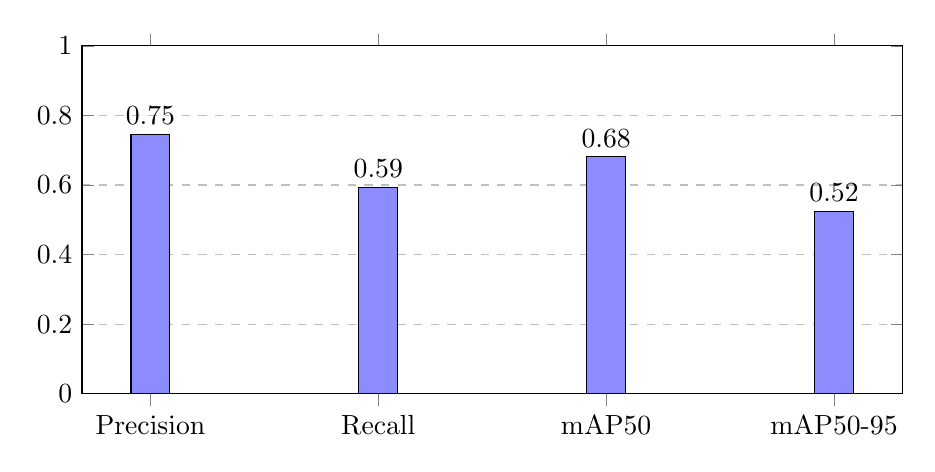
\begin{tikzpicture}
\begin{axis}[
ybar,
bar width=14pt,
width=12cm,
height=6cm,
ymin=0,
ymax=1,
symbolic x coords={Precision,Recall,mAP50,mAP50-95},
xtick=data,
ymajorgrids=true,
grid style=dashed,
nodes near coords
]
\addplot[fill=blue!45] coordinates {
(Precision,0.745)
(Recall,0.594)
(mAP50,0.681)
(mAP50-95,0.524)
};
\end{axis}
\end{tikzpicture}
\caption{Overall performance of the YOLO detection model.}
\label{fig:detgraph}
\end{figure}

\section*{Reasoning Results}
The DistilBERT reasoning model was evaluated on the scene-text dataset derived from the same real traffic images. The model performed strongly on the frequent action classes and achieved high overall accuracy. The main results are shown in Table~\ref{tab:bertresults}.

\begin{table}[H]
\centering
\caption{Reasoning model results}
\label{tab:bertresults}
\begin{tabular}{lc}
\toprule
\textbf{Metric} & \textbf{Value} \\
\midrule
Validation loss & 0.937 \\
Accuracy & 0.940 \\
Macro F1-score & 0.547 \\
Weighted F1-score & 0.932 \\
\bottomrule
\end{tabular}
\end{table}

The gap between accuracy and macro F1 is meaningful. It indicates that the model performs well on common classes but struggles on rare action labels. This is mainly due to class imbalance in the generated reasoning dataset.

Figure~\ref{fig:labeldistribution} shows the action-label distribution used during reasoning-model training.

\begin{figure}[H]
\centering
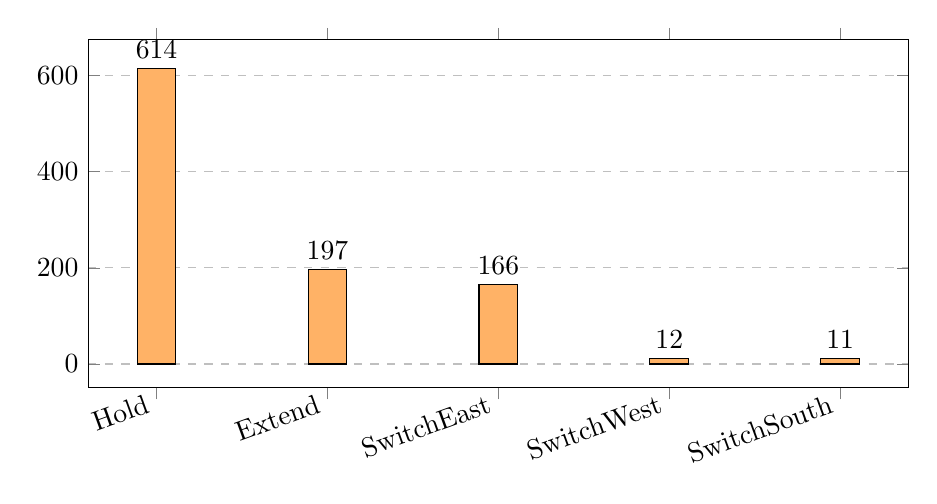
\begin{tikzpicture}
\begin{axis}[
ybar,
bar width=14pt,
width=12cm,
height=6cm,
symbolic x coords={Hold,Extend,SwitchEast,SwitchWest,SwitchSouth},
xtick=data,
x tick label style={rotate=20,anchor=east},
ymajorgrids=true,
grid style=dashed,
nodes near coords
]
\addplot[fill=orange!60] coordinates {
(Hold,614)
(Extend,197)
(SwitchEast,166)
(SwitchWest,12)
(SwitchSouth,11)
};
\end{axis}
\end{tikzpicture}
\caption{Distribution of action labels in the reasoning dataset.}
\label{fig:labeldistribution}
\end{figure}

\chapter{Discussion}
The completed work shows that the combination of computer vision and language-based reasoning is useful even in a simplified prototype setting. The object detector was able to capture the dominant vehicle types present in Indian traffic scenes, and the reasoning model was able to learn meaningful decision patterns from the generated scene descriptions.

At the same time, the project also revealed a few clear limitations. The scene abstraction remained coarse because the data was image-based rather than lane-calibrated. The reasoning labels were derived from policy logic instead of real traffic-signal telemetry. In addition, the class distribution in the decision dataset was uneven, which affected performance on rare switching classes.

Even with these limitations, the project successfully demonstrates the central idea behind the research paper. It shows that it is possible to move from raw traffic images to semantic traffic reasoning within a single workflow, and to do so using real Indian traffic data.

\chapter{Conclusion and Future Scope}
This project presented a compact multimodal traffic signal reasoning framework using YOLO and DistilBERT. The work remained focused on the essential idea of connecting perception and semantic reasoning without going too deeply into deployment complexity. The detector produced usable traffic perception results on the UVH-26 subset, and the reasoning model showed that traffic actions can be predicted from structured textual scene summaries.

The work can be extended in several ways in the future:
\begin{itemize}[leftmargin=1.5cm]
\item using a larger subset or the full UVH-26 dataset,
\item adding lane-level calibration instead of coarse scene regions,
\item incorporating emergency-vehicle handling,
\item integrating the decision stage with a traffic simulator such as SUMO,
\item and comparing the language-based reasoner with simpler numerical baselines.
\end{itemize}

Overall, the project served as a strong academic prototype and formed the basis for the associated research paper.

\chapter*{References}
\addcontentsline{toc}{chapter}{References}
\begin{enumerate}[leftmargin=1cm]
\item J. Redmon, S. Divvala, R. Girshick, and A. Farhadi, ``You Only Look Once: Unified, real-time object detection,'' in \textit{Proceedings of CVPR}, 2016.
\item J. Devlin, M. W. Chang, K. Lee, and K. Toutanova, ``BERT: Pre-training of deep bidirectional transformers for language understanding,'' in \textit{Proceedings of NAACL-HLT}, 2019.
\item V. Sanh, L. Debut, J. Chaumond, and T. Wolf, ``DistilBERT, a distilled version of BERT: smaller, faster, cheaper and lighter,'' arXiv:1910.01108, 2019.
\item B. A. Paranjape and A. A. Naik, ``DATS\_2022: A versatile Indian dataset for object detection in unstructured traffic conditions,'' \textit{Data in Brief}, 2022.
\item R. Kumar, D. S. Reddy, and P. Rajalakshmi, ``DriveIndia: An object detection dataset for diverse Indian traffic scenes,'' arXiv, 2025.
\item A. Sharma et al., ``The Urban Vision Hackathon dataset and models: Towards image annotations and accurate vision models for Indian traffic,'' arXiv, 2025.
\item S. Zhang et al., ``TrafficGPT: Viewing, processing and interacting with traffic foundation models,'' \textit{Transport Policy}, 2024.
\item M. Movahedi and J. Choi, ``The crossroads of LLM and traffic control: A study on large language models in adaptive traffic signal control,'' \textit{IEEE Transactions on Intelligent Transportation Systems}, 2024.
\end{enumerate}

\end{document}
